\documentclass{article}

% Packages to enhance functionality
\usepackage{amsmath}     % For advanced math
\usepackage{graphicx}    % To insert images
\usepackage[margin=1in]{geometry} % To adjust page margins
\usepackage{hyperref}    % To add clickable links

\title{Exploring LaTeX Packages}
\author{A Happy Learner}
\date{\today}

\begin{document}

\maketitle
\tableofcontents


\section{Why Packages?}
Packages in LaTeX are like power-ups in a game. They add cool features to make your document smarter, prettier, and more functional!

\section{Using \texttt{amsmath}}
This package helps with beautiful math. Here are some equations:
\begin{align}
    a^2 + b^2 &= c^2 \\
    E &= mc^2 \\
    \sum_{i=1}^n i &= \frac{n(n+1)}{2}
\end{align}

\section{Using \texttt{graphicx}}
This lets us add images. Example below (you need to have \texttt{duck.png} in your folder):

\begin{center}
\includegraphics[width=0.4\textwidth]{}
\begin{figure}
    \centering
    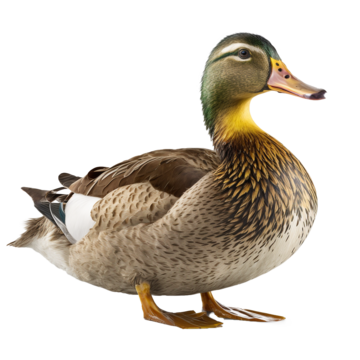
\includegraphics[width=0.5\linewidth]{session3/duck.png}
    \label{fig:enter-label}
\end{figure}
\end{center}

\section{Using \texttt{geometry}}
With this, you can control page layout easily. We used:
\begin{verbatim}
\usepackage[margin=1in]{geometry}
\end{verbatim}
It sets equal 1-inch margins all around.

\section{Using \texttt{hyperref}}
You can add clickable links and references:
\begin{itemize}
    \item Visit \href{https://www.overleaf.com}{Overleaf}
    \item Clickable section titles thanks to \texttt{\textbackslash tableofcontents}
\end{itemize}

\section{Wrap-up}
With just a few packages, your LaTeX document becomes powerful and polished. That’s the magic of LaTeX!

\end{document}
